\singlespacing  

\subsection{Neural Network Topology Motivation}

Different neural network architectures lead to different activation lifetime patterns, which directly affect the difficulty of static memory planning. In a simple sequential network, each layer consumes the output of the previous layer and produces a new activation tensor that is used shortly afterwards. As a result, tensor lifetimes are short and overlap only locally, making memory reuse relatively easy.

More complex neural network architectures introduce structures that increase memory pressure. Residual connections, commonly used in ResNet-style networks, reuse outputs from earlier layers through skip connections. These tensors must remain alive until a later merge operation, which reduces opportunities for memory reuse. Another common pattern is the multi-branch architecture, such as in Inception-style networks, where the computation splits into several parallel branches before merging the results. In this case, multiple activation tensors may exist in memory at the same time, creating more lifetime overlap. In addition, some architectures merge these branches only at a later stage. In such late-merge structures, tensors remain alive for longer periods, which increases peak memory usage.

Figure~\ref{fig:topologies} shows simplified DAG representations of the four topology patterns used in this work: sequential execution, residual connections, fork--join branching, and late-merge structures. These patterns correspond to increasing levels of tensor lifetime overlap and therefore increasing difficulty for static memory allocation.

\begin{figure}[t]
\centering

\begin{subfigure}{0.45\linewidth}
\centering
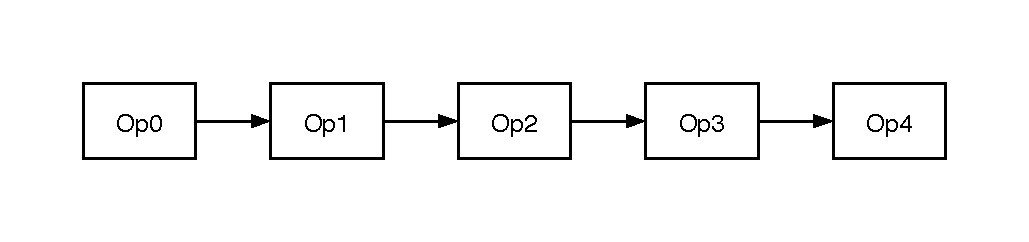
\includegraphics[width=\linewidth]{figures/sequential_topology.pdf}
\caption{Sequential}
\end{subfigure}
\hfill
\begin{subfigure}{0.45\linewidth}
\centering
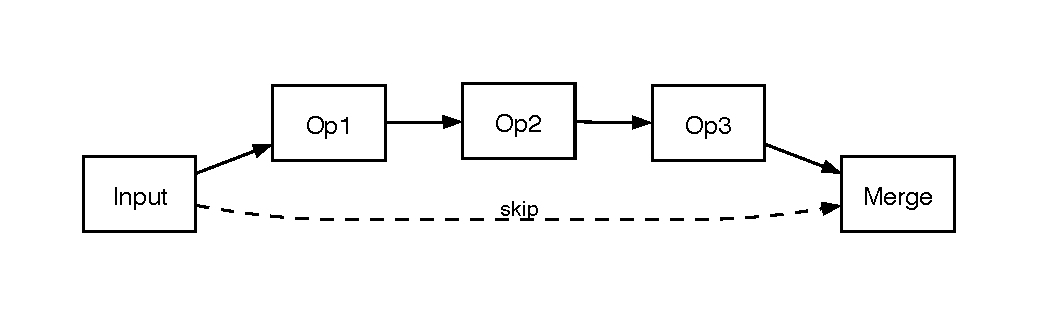
\includegraphics[width=\linewidth]{figures/residual_topology.pdf}
\caption{Residual connections}
\end{subfigure}

\vspace{0.4cm}

\begin{subfigure}{0.45\linewidth}
\centering
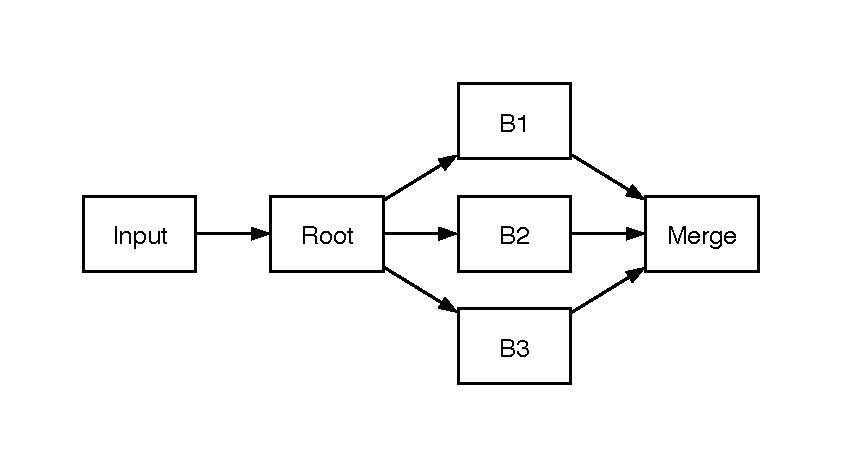
\includegraphics[width=\linewidth]{figures/forkjoin_topology.pdf}
\caption{Fork--join branching}
\end{subfigure}
\hfill
\begin{subfigure}{0.45\linewidth}
\centering
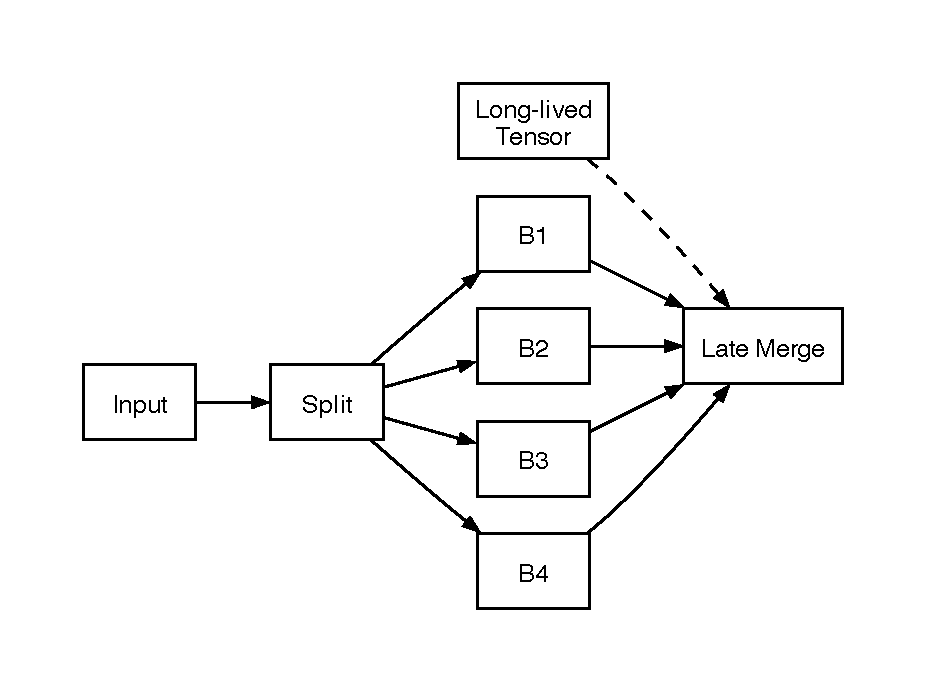
\includegraphics[width=\linewidth]{figures/latemerge_topology.pdf}
\caption{Late-merge structure}
\end{subfigure}

\caption{Representative DAG patterns used in the dataset generator:
(a) sequential execution,
(b) residual connections with skip edges,
(c) fork--join branching,
and (d) late-merge architectures.}
\label{fig:topologies}

\end{figure}

These four patterns represent increasing levels of memory allocation difficulty, from simple sequential execution to multi-branch structures with long-lived tensors. Evaluating allocation algorithms on these different structures helps us understand how network topology affects memory reuse and peak memory usage.


\subsection{Dataset Generation}

To evaluate the memory planning algorithms, we implemented a dataset generator that produces activation tensor records following the topology patterns described above. Each tensor record contains four attributes: a tensor identifier, its aligned memory size in bytes, the operator index where the tensor becomes live, and the operator index where it is last used. These attributes are sufficient to model tensor lifetimes for static memory planning.

Four topology families are generated: \textit{sequential}, \textit{residual}, \textit{fork--join}, and \textit{late-merge}. The sequential datasets represent simple chain-like execution with short tensor lifetimes. The residual datasets introduce several long-lived tensors that simulate skip connections. The fork--join datasets model multi-branch computation where tensors from different branches overlap in time. The late-merge datasets further increase the difficulty by allowing several tensors to remain alive until a late merge stage.

For each topology family, ten dataset instances are generated using different random seeds, resulting in a total of forty benchmark instances, as summarized in Table~\ref{tab:dataset}. Each instance contains approximately 12--20 tensors, depending on the topology structure. Tensor sizes are sampled from predefined ranges with small random variations and are aligned to 16-byte boundaries to reflect typical embedded memory alignment constraints.

\begin{table}[t]
\centering
\caption{Summary of generated dataset topologies}
\label{tab:dataset}
\begin{tabular}{lccc}
\hline
Topology & Instances & Tensors (approx.) & Main Feature \\
\hline
Sequential & 10 & 12--16 & Short lifetimes \\
Residual & 10 & 14--18 & Long skip tensors \\
Fork--Join & 10 & 15--20 & Branch overlap \\
Late Merge & 10 & 16--20 & Long-lived tensors \\
\hline
\end{tabular}
\end{table}